\subsection{Convolution d'image}



\begin{frame}{Une base de données plus complexe}
    \begin{block}{Deux façons différentes de faire du traitement d'image}
        \begin{itemize}
            \item L'image $28\times28$ pixels est aplatie en un vecteur de taille $784$.
            \item L'image 2D est directement prise en entrée du réseau de neurones.
        \end{itemize}
    \end{block}
    \begin{columns}
        \begin{column}{0.5\textwidth}
            \begin{figure}
                \centering
                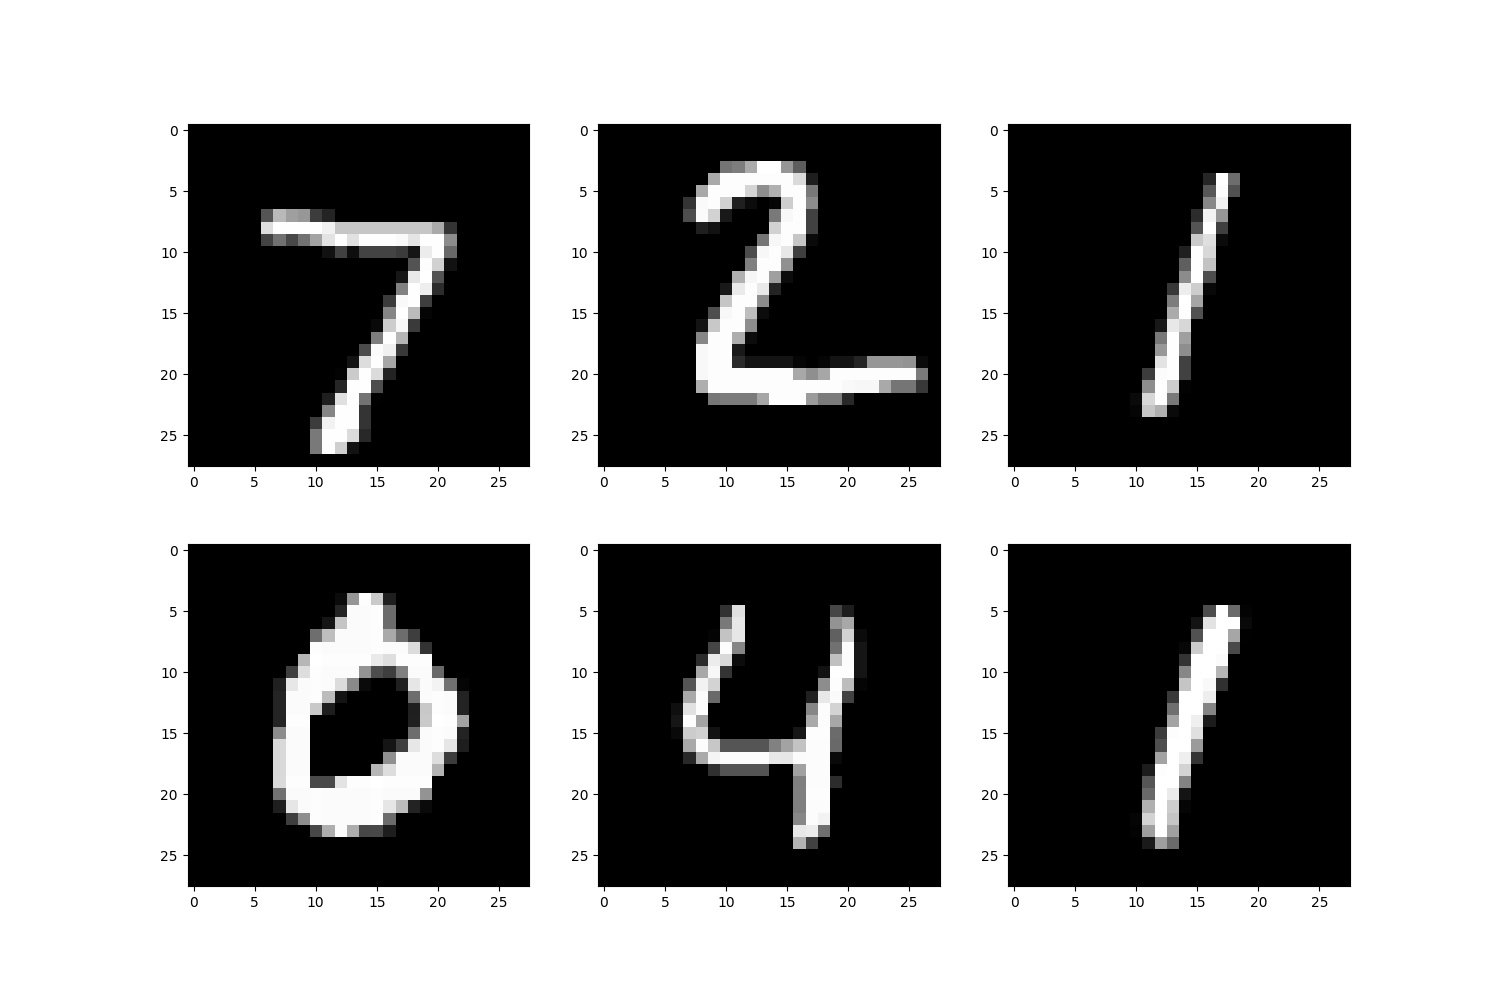
\includegraphics[width=\textwidth]{1-mnist.jpg}
                \caption{Chiffres écrits à la main}
            \end{figure}
        \end{column}
        \begin{column}{0.5\textwidth}
            \begin{figure}
                \centering
                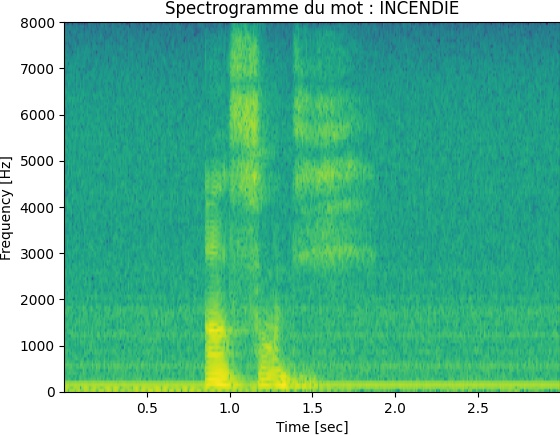
\includegraphics[width=0.9\textwidth]{1-Incendie.jpg}
                \caption{Spectrogramme}
            \end{figure}
        \end{column}
    \end{columns}
\end{frame}

\begin{frame}{La convolution d'image}
    \begin{figure}
        \centering
        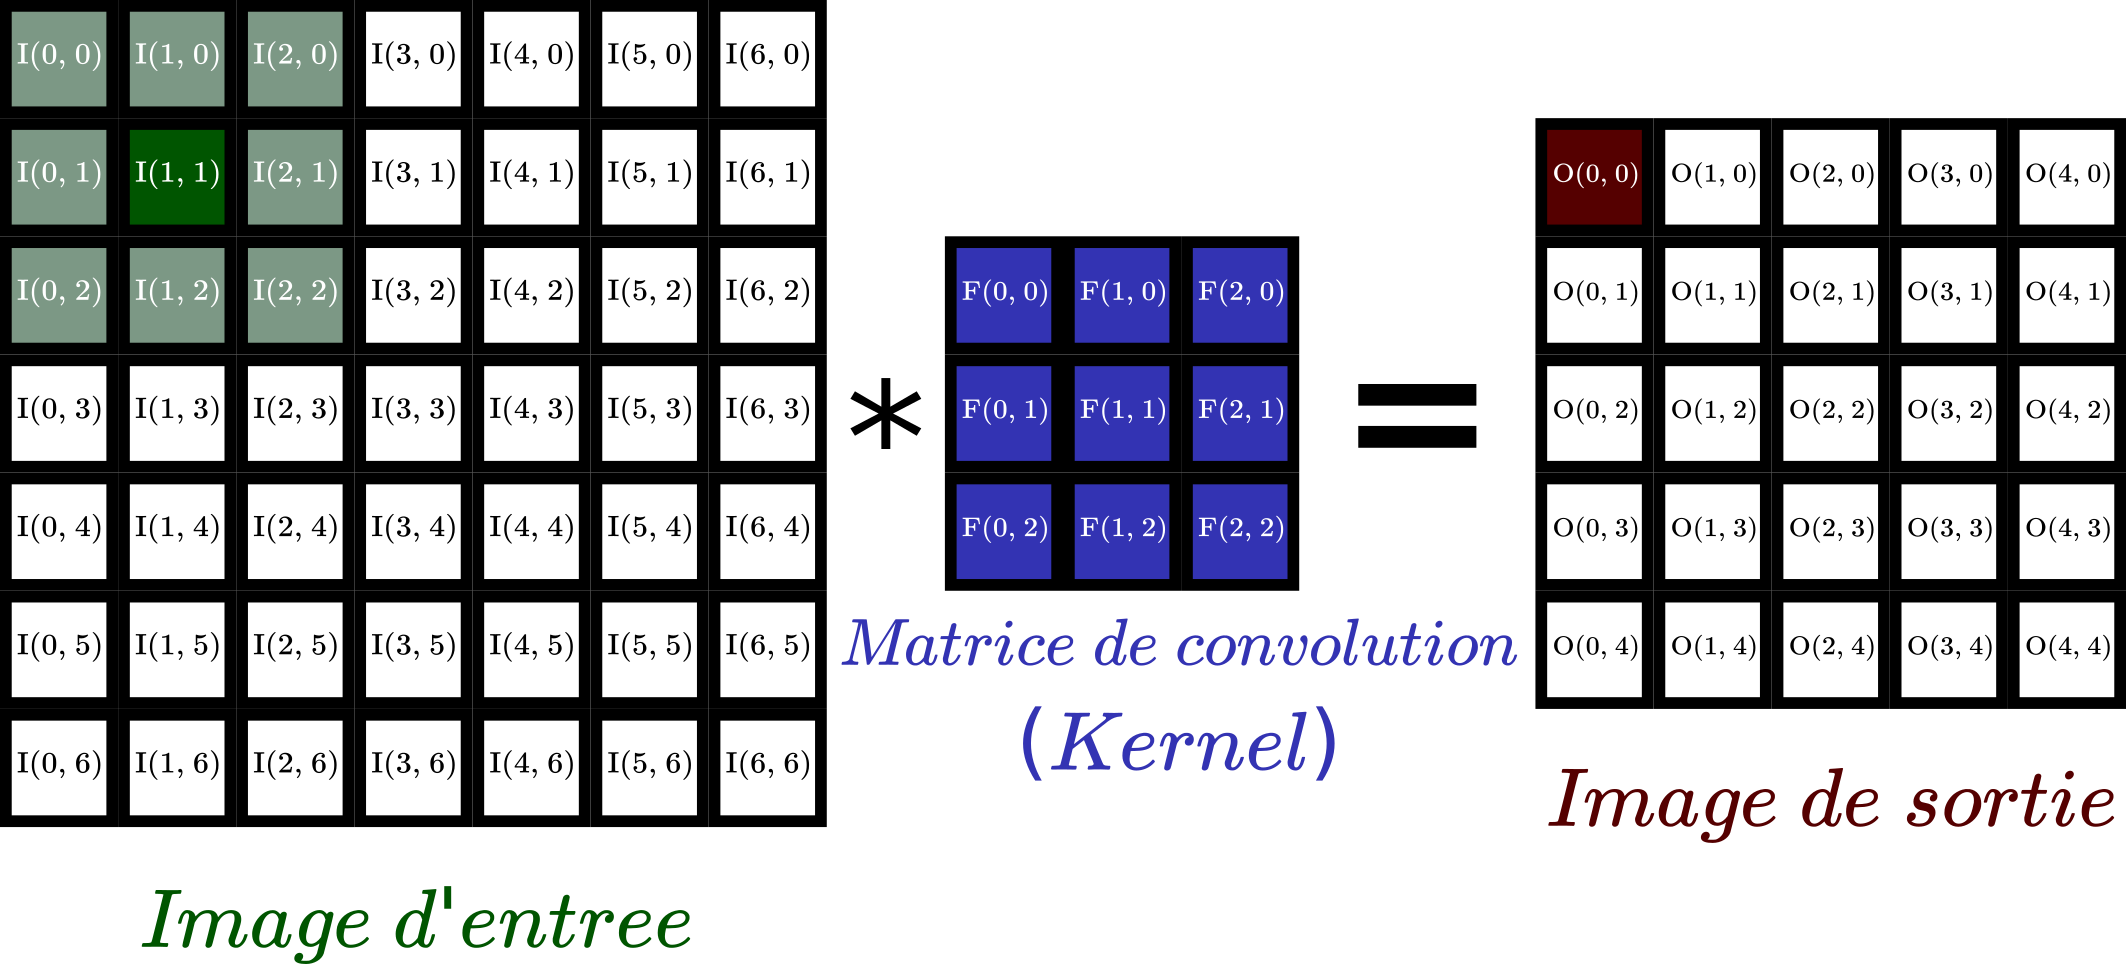
\includegraphics[width=\textwidth]{5-convolution.png}
        \centering
        \caption{Schéma de la convolution d'image $O(0, 0) = \sum_{i=0}^{2}\sum_{j=0}^{2}I(i, j)\times F(i, j)$}
    \end{figure}
\end{frame}


\begin{frame}{Un exemple de convolution d'image}
    \begin{columns}[T] % align columns
        \begin{column}{.6\textwidth}
            \begin{figure}
                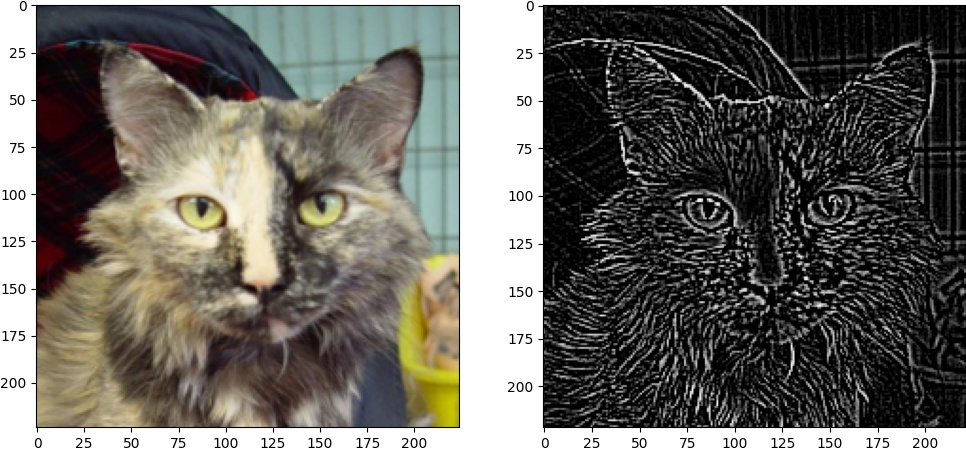
\includegraphics[width=\textwidth]{6-cat.jpg}
                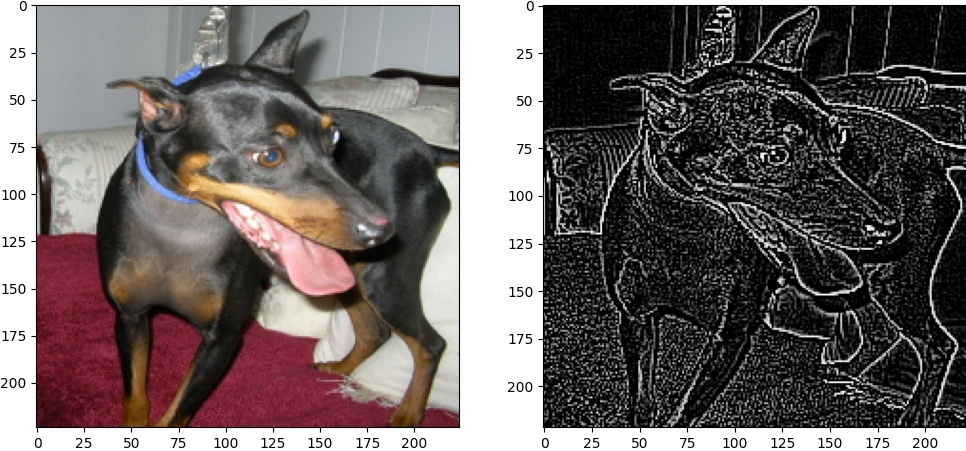
\includegraphics[width=\textwidth]{6-dog.jpg}
                \caption[]{Exemple de convolution d'image}
            \end{figure}
        \end{column}
        \begin{column}{0.35\textwidth}
            \begin{exampleblock}{Détection de contour}
                \begin{center}
                    \centering
                    $
                        F =
                        \begin{pmatrix}
                            -1 & -1 & -1 \\
                            -1 & 8  & -1 \\
                            -1 & -1 & -1
                        \end{pmatrix}
                    $
                \end{center}
            \end{exampleblock}
        \end{column}
    \end{columns}
\end{frame}


\begin{frame}{Le schéma du réseau de neurones convolutif}
    \begin{figure}
        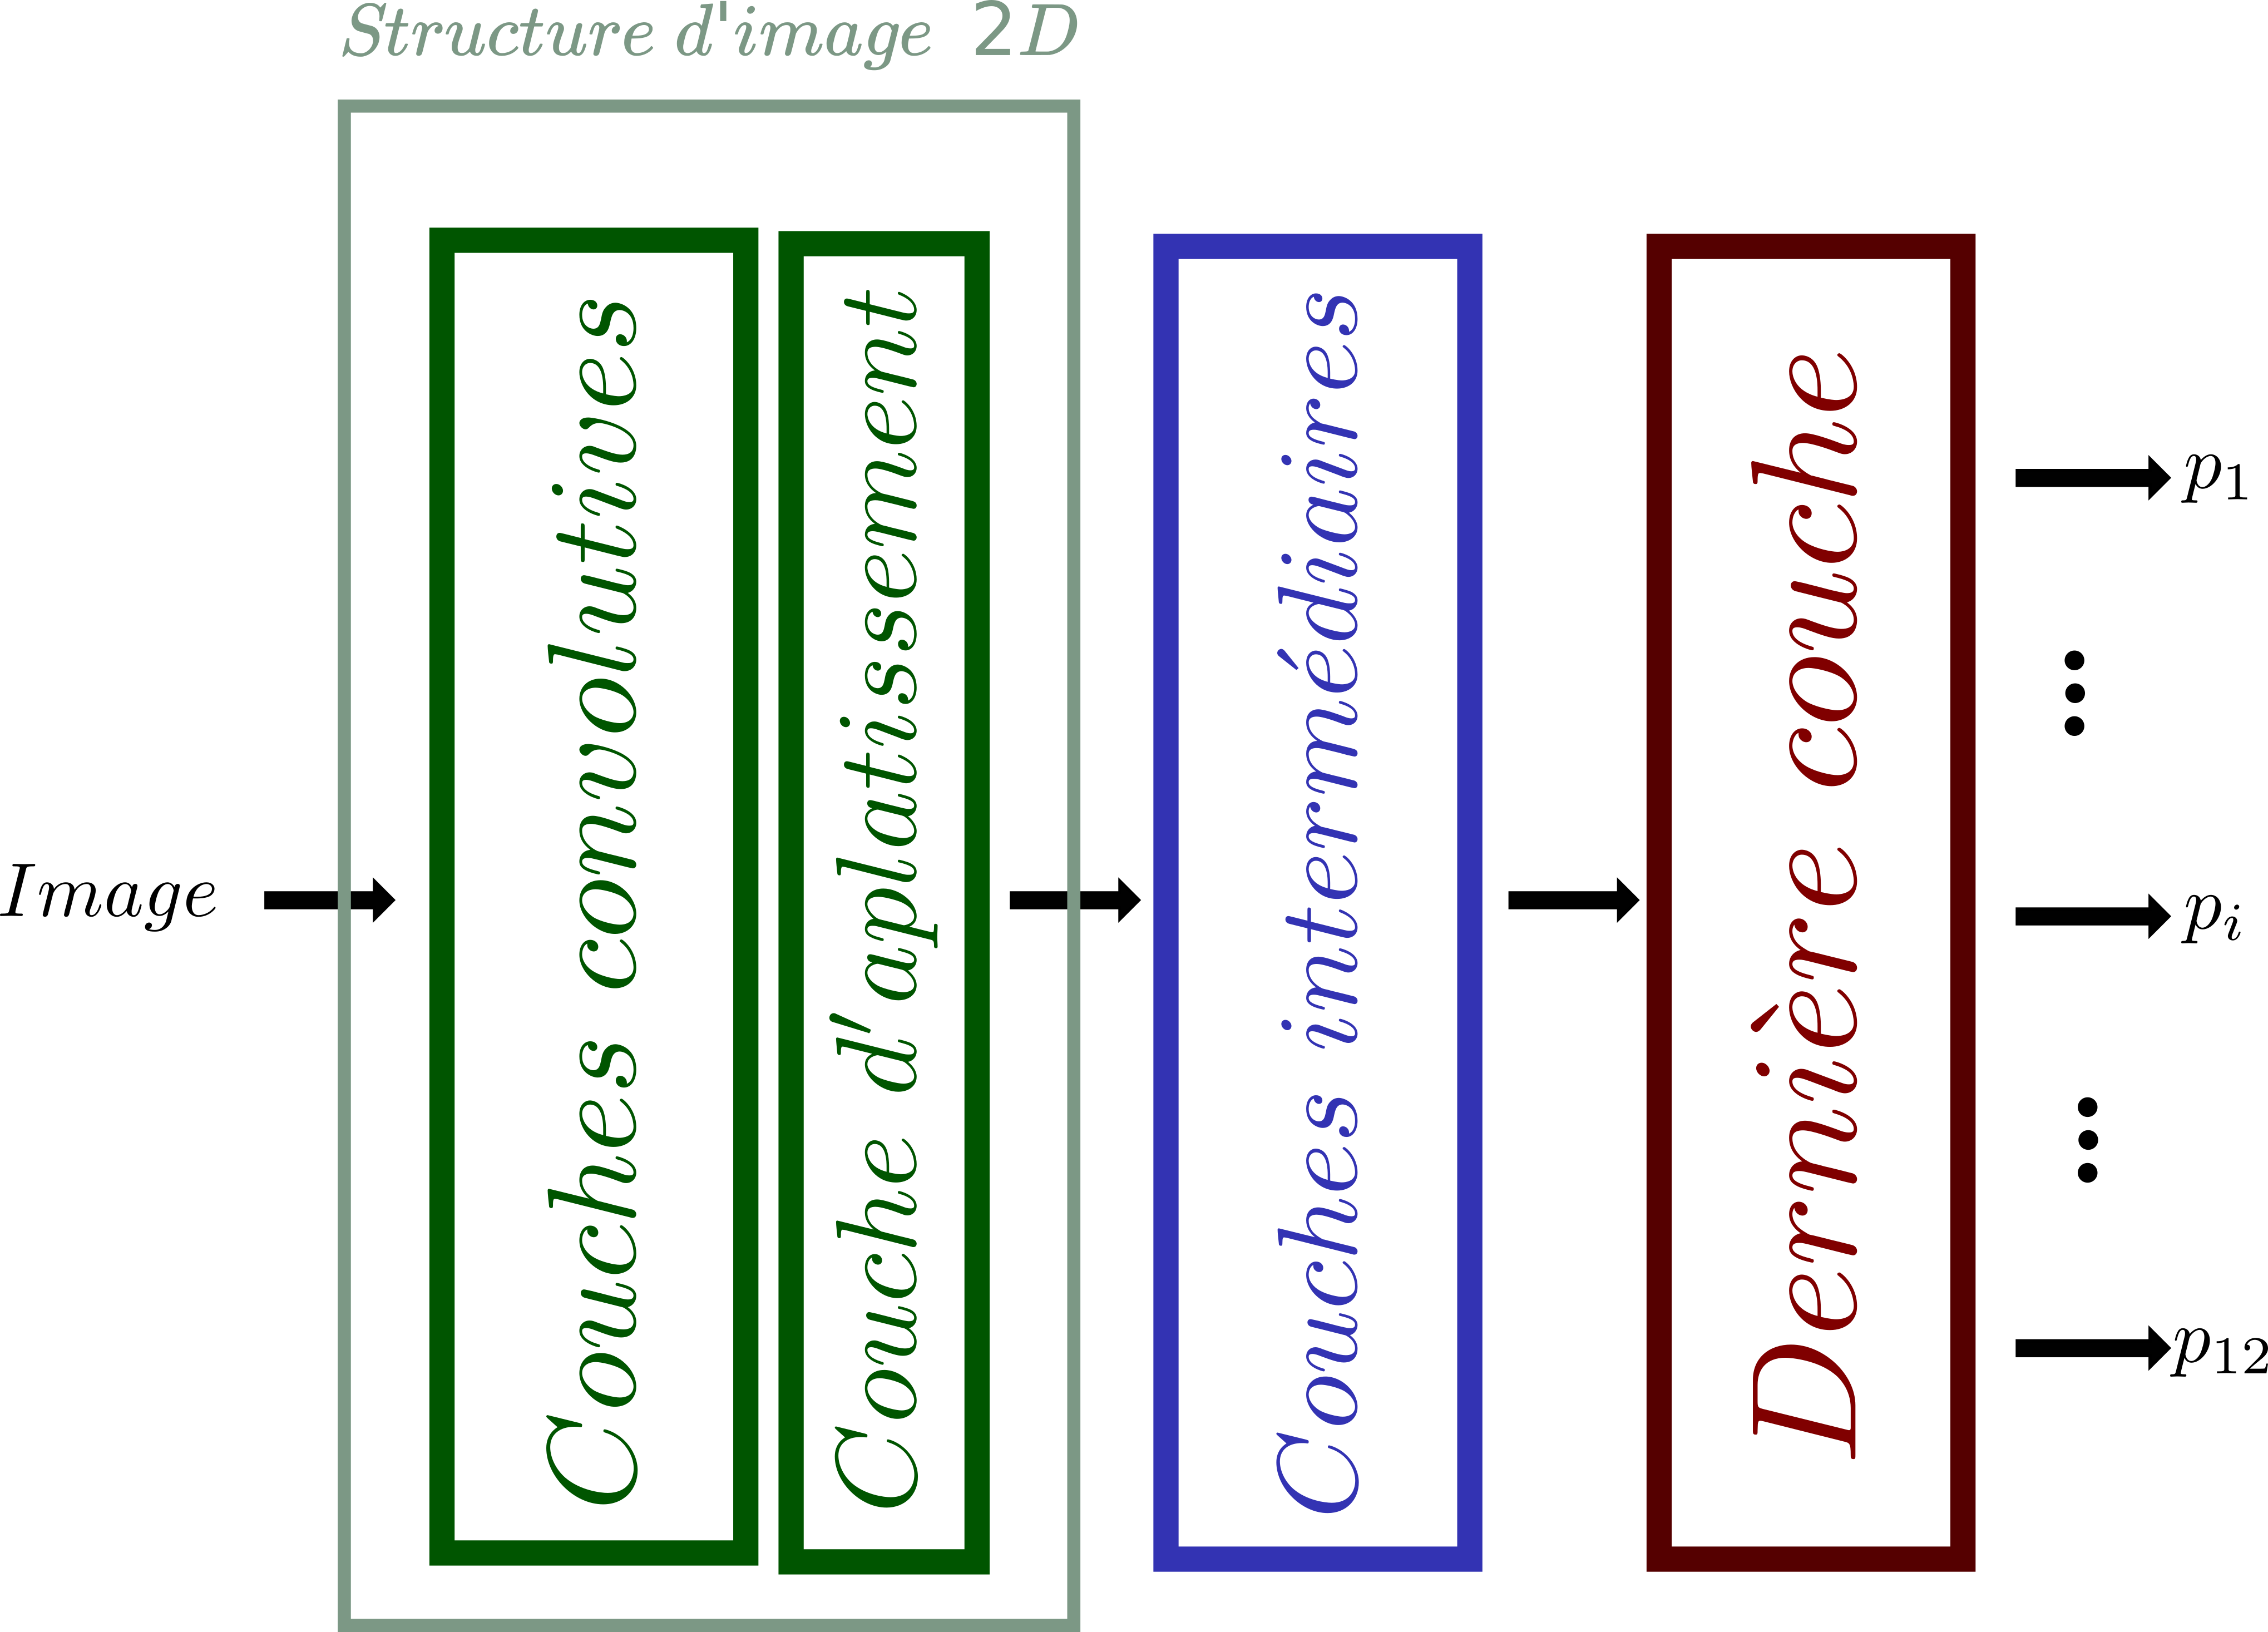
\includegraphics[height=0.7\textheight]{9-reseau convolutif.png}
        \caption[]{Schéma de réseau de neurones convolutif}
    \end{figure}
\end{frame}
